\textbf{Exemplo 1:} Sejam 
\[
J_1 = (x_1 - 1,96; \; x_1 + 1,96) \quad \text{e} \quad J_2 = \left( \bar{x} - \frac{1,96}{\sqrt{2}}, \; \bar{x} + \frac{1,96}{\sqrt{2}} \right)
\]
dois intervalos aleatórios tais que \( x_1, x_2 \sim N(\mu, 1) \) e 
\[
\bar{x} = \frac{x_1 + x_2}{2}.
\]
Encontre as probabilidades de cobertura de \( J_1 \) e \( J_2 \).

\textbf{Solução:} Temos que
\begin{align*}
P_\mu(\mu \in J_1) &= P_\mu\left( \mu \in (x_1 - 1,96; \; x_1 + 1,96) \right) \\
&= P_\mu\left( x_1 - 1,96 < \mu < x_1 + 1,96 \right) \\
&= P_\mu\left( [ \; (x_1 - \mu) < 1,96 \; ] \; \cap \; [ \; (x_1 - \mu) > -1,96 \; ] \right) \\
&= P_\mu\left( |x_1 - \mu| < 1,96 \right) \\
&= P_\mu\left( |Z| < 1,96 \right), \quad Z = x_1 - \mu \sim N(0,1) \\
&= 95\%.
\end{align*}

\begin{center}
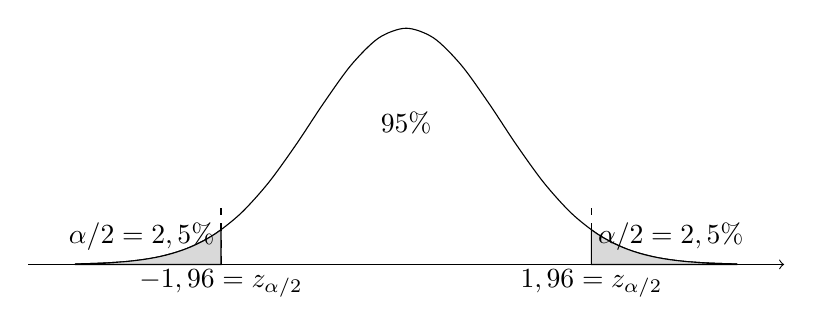
\begin{tikzpicture}[scale=1.2]
\draw[->] (-4,0) -- (4,0) node[right] {};
\draw[domain=-3.5:3.5,smooth,variable=\x,black] plot ({\x},{2.5*exp(-\x*\x/2)});
\draw[dashed] (-1.96,0) -- (-1.96,0.6);
\draw[dashed] (1.96,0) -- (1.96,0.6);
\draw[fill=gray!30] (-3.5,0) -- plot[domain=-3.5:-1.96] ({\x},{2.5*exp(-\x*\x/2)}) -- (-1.96,0) -- cycle;
\draw[fill=gray!30] (1.96,0) -- plot[domain=1.96:3.5] ({\x},{2.5*exp(-\x*\x/2)}) -- (3.5,0) -- cycle;
\node at (0,1.5) {95\%};
\node at (-2.8,0.3) {$\alpha/2 = 2,5\%$};
\node at (2.8,0.3) {$\alpha/2 = 2,5\%$};
\node at (-1.96,-0.2) {$-1,96 = z_{\alpha/2}$};
\node at (1.96,-0.2) {$1,96 = z_{\alpha/2}$};
\end{tikzpicture}
\end{center}

Da mesma forma,
\[
P_\mu(\mu \in J_2) = P_\mu\left( \mu \in \left( \bar{x} - \frac{1,96}{\sqrt{2}}, \; \bar{x} + \frac{1,96}{\sqrt{2}} \right) \right) \Rightarrow
\]